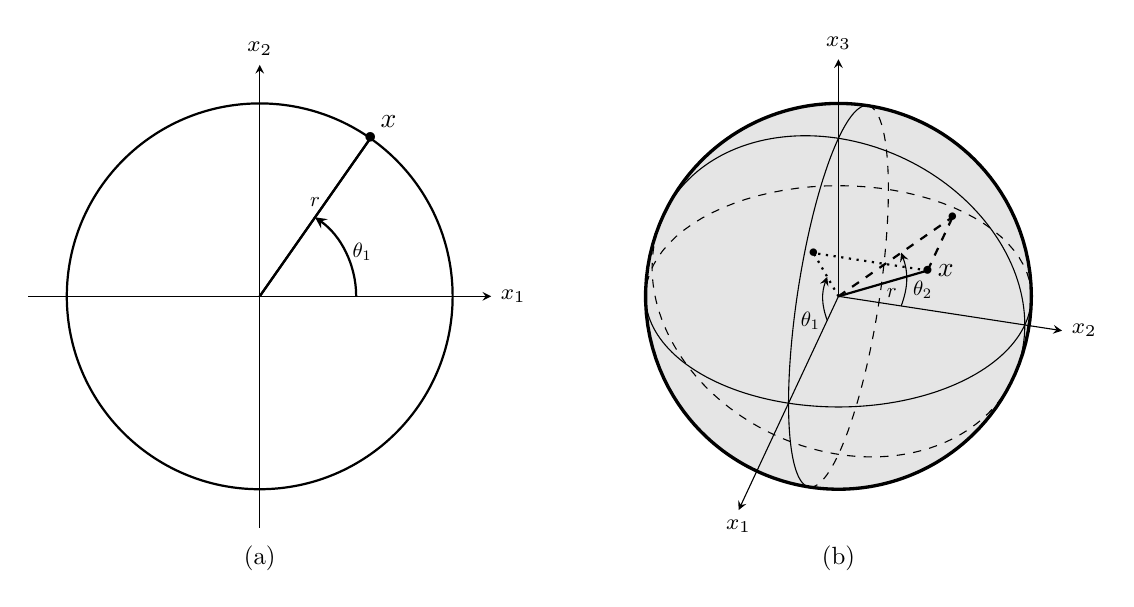
\begin{tikzpicture}[scale=.7]
\shorthandoff{>}

% CUIDADO
% Para el dibujo de la esfera, todo era hecho  en coordenadas esfericas de fisica (theta,phi)
% Para el punto x, se usan las coordenadas como en el libro, (theta_1,theta_2)
% (on dos parametrizaciones de la misma cosa...)
%
% Proyeccion para diburar un punto (x_1,x_2,x_3) teniendo en cuenta el angulo de vision
\pgfmathdeclarefunction{projx}{2}{\pgfmathparse{#1*cos(\Az)-#2*sin(\Az)}}
\pgfmathdeclarefunction{projy}{3}{\pgfmathparse{#1*sin(\Az)*sin(\El)+#2*cos(\Az)*sin(\El)+#3*cos(\El)}}


% unas definiciones para elegir el angolu de vision
\pgfmathsetmacro{\El}{35} % Elevacion
\pgfmathsetmacro{\Az}{-105}% Azimuth
%
\pgfmathsetmacro\r{3.5} % radio del circulo (d=2) y de la esfera (d=3)
%
%
% punto x para el caso d = 2
\pgfmathsetmacro\tpbi{55} % theta_1
\pgfmathsetmacro\xpbi{\r*cos(\tpbi)} % x_1
\pgfmathsetmacro\ypbi{\r*sin(\tpbi)} % x_2
%
%
% punto x para el caso d = 3
\pgfmathsetmacro\tu{60} % theta_1 punto x
\pgfmathsetmacro\td{45} %theta_2 punto x
\pgfmathsetmacro\xp{\r*cos(\tu)} % x_1 de x
\pgfmathsetmacro\yp{\r*sin(\tu)*cos(\td)} % x_2 de x
\pgfmathsetmacro\zp{\r*sin(\tu)*sin(\td)} % x_3 de x
%\pgfmathsetmacro\xp{\rp*cos(\tp)*cos(\pp)} % x_1 de x
%\pgfmathsetmacro\yp{\rp*sin(\tp)*cos(\pp)} % x_2 de x
%\pgfmathsetmacro\zp{\rp*sin(\pp)} % x_3 de x
%
%
% funcion permitiendo calcular phi(theta) dando la linea de cumbre
\pgfmathdeclarefunction{phicr}{1}{\pgfmathparse{
atan((sin(#1)*cos(\Az)+cos(#1)*sin(\Az))/(tan(\El)))
}}
%
% ====================================================================
%
% -----------------
% | Circulo d = 2 |
% -----------------
%
\begin{scope}
%
%  axes
% ------
%
\draw[>=stealth, ->] ({-1.2*\r},0)--({1.2*\r},0) node[right] {\footnotesize $x_1$};
\draw[>=stealth, ->] (0,{-1.2*\r})--(0,{1.2*\r}) node[above] {\footnotesize $x_2$};
%
%
%  Circulo
% --------
%
\draw[thick] (0,0) circle (\r);
%
%\draw (\r,0) node[below]{$r$};
%
%
%  punto x, r, theta_1
% --------------------
%
\draw[thick] (0,0) -- (\xpbi,\ypbi) node[scale=.9]{$\bullet$};
\draw[thick] (0,0) -- (\xpbi,\ypbi) node[above right]{$\boldsymbol{x}$};
\draw ({\xpbi/2},{1.05*\ypbi/2}) node[above,scale=.75]{$\boldsymbol{r}$};
\draw[->,>=stealth,thick] ({\r/2},0)  arc (0:\tpbi:{\r/2});
\draw ({\r*cos(\tpbi/2)/2},{\r*sin(\tpbi/2)/2}) node[right,scale=.75] {$\boldsymbol{\theta_1}$};
%
\node at (0,{-\r-1.25}) [scale=.9]{(a)};
\end{scope}
%
%
% ====================================================================
%
% ----------
% | Esfera |
% ----------
%
\begin{scope}[xshift=10.5cm]
%
%
%  angulo de visibilidad
% -----------------------
%
\pgfmathsetmacro\tv{-\Az}
%
%
% Axes
% -----
%
\draw[>=stealth, ->] (0,0)--({projx(\r*2,0)},{projy(\r*2,0,0)}) node[below]
{\footnotesize $x_1$};
\draw[>=stealth, ->] (0,0)--({projx(0,\r*1.2)},{projy(0,\r*1.2,0)}) node[right]
{\footnotesize $x_2$};
\draw[>=stealth, ->] (0,0)--(0,{projy(0,0,\r*1.5)}) node[above]
{\footnotesize $x_3$};
%
%
% Esfera
% ------
%
% interior de la esfera / linea de cumbre
\filldraw[very thick, domain=-\Az:-\Az+360, variable=\t, samples=180, fill opacity=.1]
plot ({projx(\r*cos(\t)*cos(phicr(\t)),\r*sin(\t)*cos(phicr(\t)))} , 
      {projy(\r*cos(\t)*cos(phicr(\t)),\r*sin(\t)*cos(phicr(\t)),\r*sin(phicr(\t)))});
%
% Ecuador (para visualisar la esfera), dado por phi = 0:
% parte visible
\draw[domain=-\Az+180:-\Az+360, variable=\t, samples=90]
plot ({projx(\r*cos(\t),\r*sin(\t))},{projy(\r*cos(\t),\r*sin(\t),0)});
%
% partie invisible
\draw[dashed, domain=-\Az:-\Az+180, variable=\t, samples=45]
plot ({projx(\r*cos(\t),\r*sin(\t))},{projy(\r*cos(\t),\r*sin(\t),0)});
%
% Linea de longitud para que se vea bien la surfaza: theta = 0 y 90
% parte visible theta = 0
\draw[domain=phicr(0):phicr(0)+180, variable=\p, samples=90]
plot ({projx(\r*cos(\p),0)},{projy(\r*cos(\p),0,\r*sin(\p))});
%
% partie escondida theta = 0
\draw[dashed, domain=phicr(0)+180:phicr(0)+360, variable=\p, samples=90]
plot ({projx(\r*cos(\p),0)},{projy(\r*cos(\p),0,\r*sin(\p))});
%
% parte visible theta = 90
\draw[domain=phicr(90):phicr(90)+180, variable=\p, samples=90]
plot ({projx(0,\r*cos(\p))},{projy(0,\r*cos(\p),\r*sin(\p))});
%
% partie escondida theta = 90
\draw[dashed, domain=phicr(90)+180:phicr(90)+360, variable=\p, samples=90]
plot ({projx(0,\r*cos(\p))},{projy(0,\r*cos(\p),\r*sin(\p))});
%
%
% Punto
% ------
%
%
% Posicion del punto x
\draw[thick] (0,0) --
({projx(\xp,\yp},{projy(\xp,\yp,\zp)})
node[scale=.75]{$\bullet$};
%
\draw[thick]
({projx(\xp,\yp},{projy(\xp,\yp,\zp)})
node[right]{$\boldsymbol{x}$};
%
%
% proyecciones para poner los angulos
% x1 = 0
%\draw[thick,dashed] ({projx(\xp,\yp},{projy(\xp,\yp,\zp})--({projx(0,\yp},{projy(0,\yp,\zp});
%\draw[thick,dashed] (0,0)--({projx(0,\yp},{projy(0,\yp,\zp});
%\draw[thick,dashed] ({projx(0,\yp},{projy(0,\yp,0})--({projx(0,\yp},{projy(0,\yp,\zp});
%
%
% notacion del radio
\pgfmathsetmacro{\propr}{.6} % distancia del radio para anotar "r"
\draw ({projx(\propr*\xp,\propr*\yp},{projy(\propr*\xp,\propr*\yp,\propr*\zp})
node[below,scale=.75] {$\boldsymbol{r}$};
%
%
% notacion del angulo theta_1
\pgfmathsetmacro{\proptu}{.45} % "radio" para dibujar el angulo
\draw[thick,dotted] ({projx(\xp,\yp},{projy(\xp,\yp,\zp})--({projx(\xp,0},{projy(\xp,0,\zp});;% proy x2=0
\draw[thick,dotted] (0,0)--({projx(\xp,0},{projy(\xp,0,\zp}) node[scale=.7]{$\bullet$};% proy x2=0
\draw[->,>=stealth]
({projx(\proptu*\xp,0)},{projy(\proptu*\xp,0,0)}) to [bend left=20]
node[pos=0,left,scale=.75] {$\boldsymbol{\theta_1}$}
({projx(\proptu*\xp,0)},{projy(\proptu*\xp,0,\proptu*\zp)});
%
%
% notacion del angulo theta_2
\pgfmathsetmacro{\propp}{.55} % "radio" para dibujar el angulo
\draw[thick,dashed] ({projx(\xp,\yp},{projy(\xp,\yp,\zp})--({projx(0,\yp},{projy(0,\yp,\zp});;% proy x1=0
\draw[thick,dashed] (0,0)--({projx(0,\yp},{projy(0,\yp,\zp}) node[scale=.7]{$\bullet$};% proy x1=0
\draw[->,>=stealth]
({projx(0,\propp*\yp)},{projy(0,\propp*\yp,0)}) to [bend right=20]
node[pos=0.3,right,scale=.75] {$\boldsymbol{\theta_2}$}
({projx(0,\propp*\yp)},{projy(0,\propp*\yp,\propp*\zp)});
%
\node at (0,{-\r-1.25}) [scale=.9]{(b)};
\end{scope}
%
\end{tikzpicture}
